\section{Stochastic Dominance Analysis and Behavioral Implications}

In this final empirical exercise, we compare the full return distributions of the Robinhood portfolio and the market benchmark using nonparametric stochastic dominance tests.  
A second-order stochastic dominance (SSD) result in favor of the market would imply that \emph{every} risk-averse investor 
(including but not restricted to all CRRA preferences with $\gamma>0$) strictly prefers the market's payoff to that of the Robinhood strategy.

\subsection{Methodology}
We first estimate the empirical cumulative distribution functions (CDFs) of daily returns for the two portfolios.  Let
\begin{equation}    
    F_{p}(r) \;=\; \frac{1}{T}\sum_{t=1}^{T}\mathbf{1}\{r_{p,t}\le r\},
    \quad
    F_{m}(r) \;=\; \frac{1}{T}\sum_{t=1}^{T}\mathbf{1}\{r_{m,t}\le r\},
\end{equation}
where $r_{p,t}$ and $r_{m,t}$ are the portfolio and market returns on day $t$.  

To analyse whether the portfolio is preferred over the market we employ two different tests.
First-order stochastic dominance (FSD) holds if $F_{p}(r)\le F_{m}(r)$ for all $r$; 
second-order stochastic dominance (SSD) holds if
\begin{equation}    
    G_{p}(r) \;\equiv\;\int_{-\infty}^{r}F_{p}(x)\,dx
    \quad\text{and}\quad
    G_{m}(r)\;\equiv\;\int_{-\infty}^{r}F_{m}(x)\,dx
\end{equation}

satisfy $G_{p}(r)\le G_{m}(r)$ for all $r$.


\subsection{Results}
\subsubsection{Rolling-Horizon SSD}
\paragraph{Comparing Robinhood Portfolios}
Across non-overlapping horizons of 1, 5, 30, and 120 trading days—as well as the full 563-day sample—we compute for each return series the empirical CDFs $F_{\mathrm{Mine}}(r)$ and $F_{\mathrm{Fedyk}}(r)$, their integrals $G_{\mathrm{Mine}}(r)$ and $G_{\mathrm{Fedyk}}(r)$, and the fraction of evaluation points satisfying  
\begin{equation}
    G_{\mathrm{Fedyk}}(r)\;\le\;G_{\mathrm{Mine}}(r),
\end{equation}
which indicates Fedyk's second-order stochastic dominance over the portfolio I built.  
This support fraction falls monotonically with the horizon: it exceeds 98 \% at the 1- and 5-day horizons, drops below 1 \% at 30 days, only rebounds to about 6 \% at 120 days, and reaches 0 \% over the full period.  
These findings show that Fedyk's SSD advantage becomes increasingly stronger at longer horizons, making it preferred by every risk-averse investor.
This relation even becomes a first-order stochastic dominance when accounting for cumulative returns, as can be easily seen from plot.

\begin{figure}[H]
    \centering
    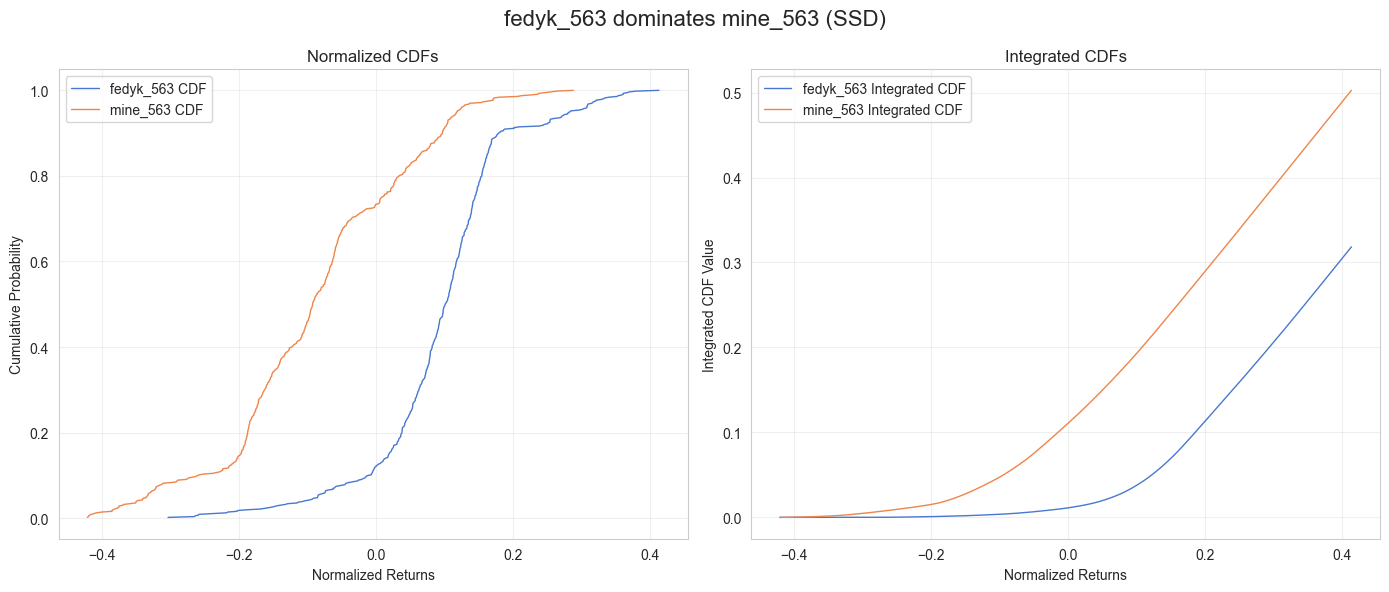
\includegraphics[width=0.8\linewidth]{../images/risk/fsd_fedyk_mine.png}
    \caption{FSD Between the Robinhood Portfolios.}
    \label{fig:fsd_fedyk_mine}
\end{figure}    


\paragraph{Comparing Robinhood to Broad-Market Proxies}  
We use the Fedyk portfolio as a conservative benchmark for comparison. 
Its demonstrated dominance over our custom Robinhood strategy across horizons makes it an especially stringent benchmark: 
if our portfolio cannot overcome Fedyk's advantage, it would be even harder to outperform true market indices at longer holding periods.

Having established that the Fedyk portfolio second-order stochastically dominates our Robinhood strategy as the length of the horizon increases, 
we now benchmark against three widely-used market proxies: the S\&P 500 ETF (VOO), the global all-world ETF (VT), and the Fama French market index (results for which are nearly identical to VOO).

At the 1- and 5-day horizons, all three market indices exhibit overwhelming SSD dominance over our Robinhood portfolio, each with over 97\% of evaluation points satisfying
\begin{equation}
    G_{\mathrm{proxy}}(r) \leq G_{\mathrm{RH}}(r).
\end{equation}

By the 30-day horizon, this support fraction declines to approximately 92\% for the S\&P 500 and 90\% for the all-world ETF, while the Fama French index mirrors the S\&P 500's trajectory. 
Extending to 120 days, the S\&P 500 retains complete dominance (100\% of points), whereas the all-world ETF's dominance share falls to about 83\%. 
Over the full 563-day sample, the S\&P 500 continues to second-order dominate Robinhood, while the all-world ETF shows only weak support ($\approx$ 8\%).
Only the S\&P 500 (VOO) and the Fama French market index preserve dominance in the long-run payoff distribution.

In other words, whether we compare the portfolio I built against the Fedyk portfolio or traditional market indices, the second-order stochastic dominance over our Robinhood strategy is nearly universal at intraday and weekly horizons. 
Our approach to building the Robinhood portfolio, fails SSD also against the World ETF at longer horizons.

\subsubsection{All-Pairs Analysis}
Our analysis now turns to the all-pairs dataset constructed according to Equation \ref{eq:allpairs_return}, which computes returns across all possible entry-exit point combinations. 
As previously established in Section \ref{sec:allpairs}, CRRA preference analysis indicates that only investors with extreme risk-seeking preferences would derive greater utility from the Robinhood portfolio compared to market indices.

These conclusions are strongly supported by stochastic dominance tests, with some cases demonstrating first-order dominance. 
When evaluating Fedyk's Robinhood portfolio against market proxies, we find the S\&P 500 and Fama French market index exhibit clear second-order stochastic dominance. 
The world ETF (VT) achieves dominance over 96\% of evaluation points, falling short of full dominance by only a marginal 4\%. 
These results hold more strongly when using our alternative Robinhood portfolio construction method, where all three market proxies demonstrate complete second-order dominance.

The pre-pandemic subsample (through February 2020) reveals even more pronounced results in favor of market indices. 
Fedyk's portfolio fails second-order dominance under all market proxies during this period. 
Notably, the Fama French index achieves first-order stochastic dominance, while the S\&P 500 and world ETF narrowly miss complete first-order dominance by merely 0.17\% and 5.92\% of evaluation points respectively. 

\begin{figure}[H]
    \centering
    \subfloat[S\&P 500]{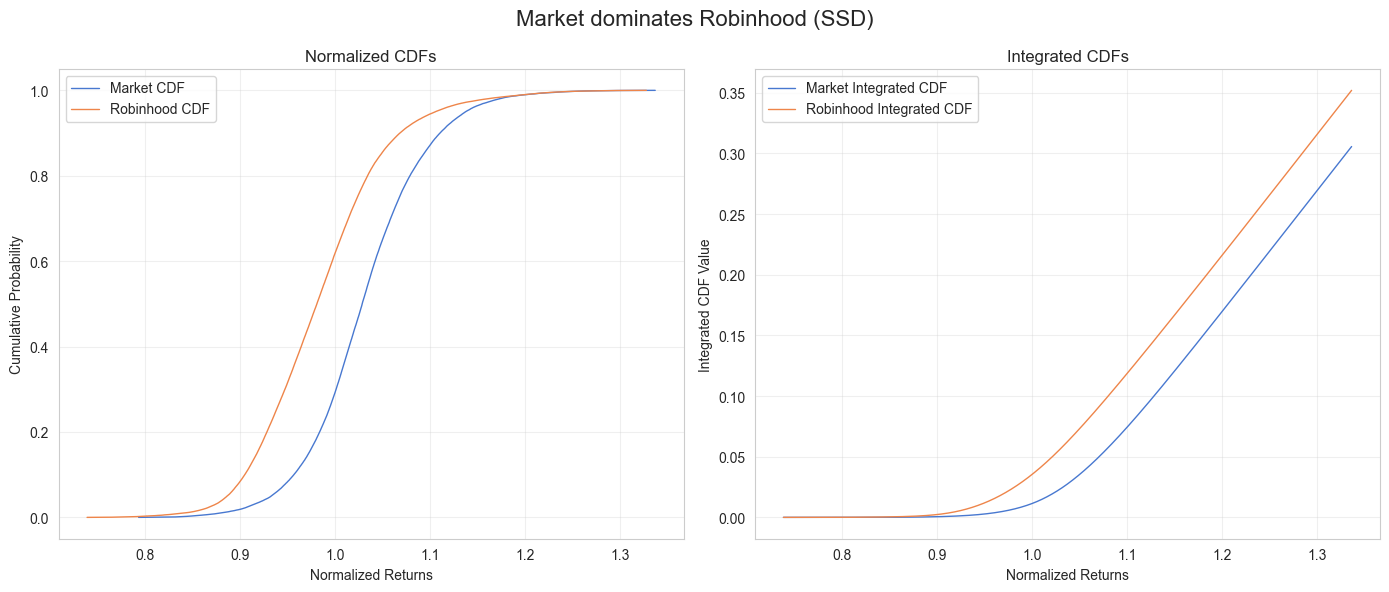
\includegraphics[width=0.48\textwidth]{../images/risk/ssd_wealth_voo_before.png}}
    \hfill
    \subfloat[World ETF]{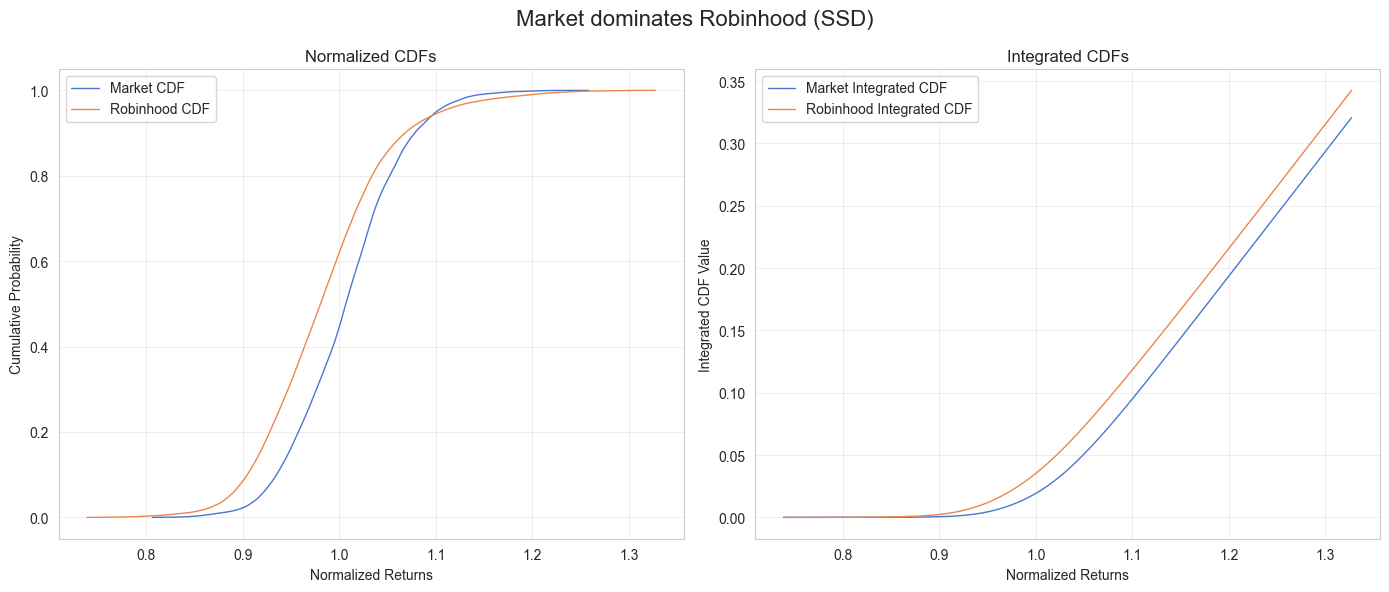
\includegraphics[width=0.48\textwidth]{../images/risk/ssd_wealth_vt_before.png}}
    \caption{Second-order stochastic dominance tests comparing Fedyk's Robinhood portfolio to market indices (pre-pandemic period through February 3, 2020).}
    \label{fig:cutoff_all_sidebyside}
\end{figure}

Our alternative Robinhood portfolio construction shows even stronger results, demonstrating first-order dominance across all three market proxies in this period.
The economic implications of these findings are particularly striking. 
For any Robinhood investor selecting entry and exit points at random, the revealed preferences would appear economically irrational - the Robinhood portfolio either suffers first-order stochastic dominance or comes remarkably close to this threshold. 
The second-order dominance results further indicate that all risk-averse investors, regardless of their specific utility function form, would have been better served by market indices. 
These results hold particular significance when considering the pre-pandemic period, where market dominance appears most pronounced.

\subsubsection{A Proof of Irrationality?}
Our analysis reveals a fundamental contradiction in Robinhood investors' revealed preferences. 
Building on the risk aversion estimates from Section~\ref{sec:gamma_estimates} (Table~\ref{tab:gamma_implied}), where we found strictly positive $\gamma$ values in 95\% confidence intervals for daily and weekly returns, we now confront these findings with stochastic dominance tests. 
This creates an irreconcilable tension: while Robinhood investors exhibit risk-averse preferences through positive $\gamma$ estimates, their chosen portfolios fail to satisfy basic rationality requirements when compared to market alternatives.

The contradiction emerges most sharply at weekly horizons. 
Despite estimated risk aversion parameters ($\hat{\gamma} > 0$) that should favor market indices under second-order stochastic dominance (SSD), we find that the Fama French market index demonstrates unambiguous SSD over both Robinhood portfolios, 
and S\&P 500 and world ETF (VT) achieve SSD over 95-99\% of evaluation points.
This implies that even the most conservative specification of risk-averse preferences would favor market indices over Robinhood strategies, directly contradicting the investors' actual portfolio choices.

The tension persists across all horizons: Daily returns show 95-98\% SSD support for market dominance, monthly returns reveal comprehensive market dominance (90.7-100\% SSD support), and only a small fraction of monthly $\hat{\gamma}$ estimates dip below zero.

\begin{figure}[H]
    \centering
    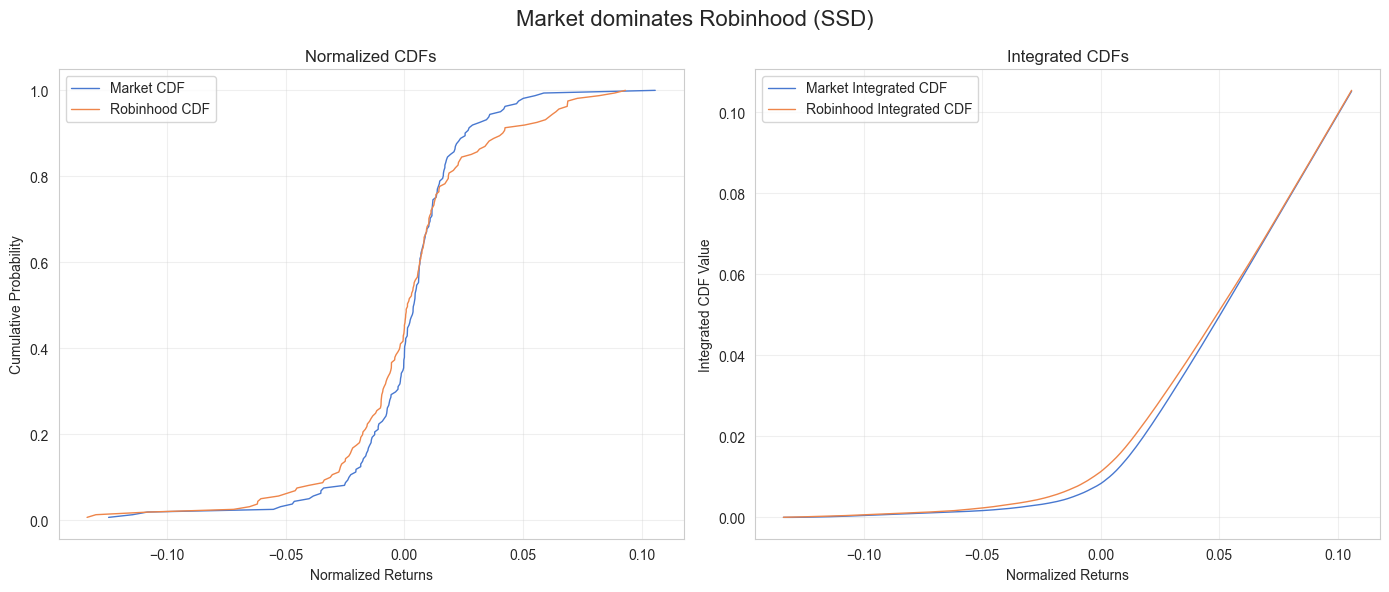
\includegraphics[width=0.8\linewidth]{../images/risk/ssd_number_5d_mkt.png}
    \caption{SSD of the Market over the Robinhood Portfolio.}
    \label{fig:fsd_fedyk_mine}
\end{figure}    

These results present an inescapable conclusion: Robinhood investors' portfolio choices cannot be rationalized through standard risk-return tradeoffs. 
The combination of (1) positive estimated risk aversion and (2) market dominance across SSD tests creates a paradox that only resolves if we reject the premise of fully rational investors.
Even under generous assumptions about return aggregation, the evidence consistently challenges the rationality hypothesis.

Our findings suggest that non-standard preferences or behavioral factors, such as lottery-seeking behavior, attention-driven trading, or misunderstanding of statistical dominance, must drive these investment decisions. 
The persistence of this contradiction across multiple methodologies (CRRA estimation, SSD tests, and temporal subsamples) makes it particularly robust to alternative explanations.


\subsection{Implications for Investor Behavior}

Our nonparametric stochastic-dominance tests deliver a clear verdict: across multiple return horizons and market proxies, the broad market consistently second-order stochastically dominates the Robinhood strategy for short-term horizons, and at monthly and longer horizons the S\&P 500 (VOO) in particular preserves that dominance where other proxies fade.  
Because SSD implies preference by every risk-averse investor (all CRRA utilities with $\gamma>0$), these results extend and reinforce our earlier finding—based on risk aversion estimation—that retail investors exhibit positive risk aversion yet hold a portfolio that no rational, CRRA-maximizer would choose.  

Taken together, the risk aversion implied by $\alpha$ and stochastic-dominance evidence point to a fundamental disconnect between normative decision rules and observed retail behavior.  
Even though our bootstrap-corrected GMM estimates uncover strictly positive—and economically plausible—risk-aversion parameters at daily and weekly frequencies, 
the SSD tests show that any such risk-averse investor would uniformly prefer the market portfolio.  
The persistence of sub-optimal, under-diversified strategies therefore cannot be attributed to risk-aversion alone.

Instead, these findings call for behavioral explanations: investors may succumb to overconfidence in their timing ability, confirmation bias in interpreting past returns, or an illusion of control over individual trades.  
Such biases can sustain a self-confirming equilibrium, in which retail traders overweight episodes of success and dismiss losses as noise, reinforcing the belief that their custom portfolio offers an edge—even when the broad market outperforms on every risk-averse criterion.
By combining both approaches, we provide robust evidence that, despite genuine risk aversion, retail investors systematically deviate from the optimal market portfolio—highlighting the crucial role of behavioral frictions in real-world decision-making.  
